
\chapter{Metodología}
\label{cap:Metodologia}

El objetivo de este capítulo será el describir la metodología aplicada al desarrollo de este Trabajo Fin de Máster.

Se define como metodología, según la RAE \cite{rae-metodologia}, como el conjunto de métodos y pasos seguidos seguidos para una investigación o estudio sobre algo concreto. Esta definición, que en el contexto de la informática puede parecer algo abstracta, se puede reescribir como la división de un trabajo complejo en diversas partes (\emph{fases}) más simples, de forma que éstas sean aplicables a cualquier tipo de proyecto similar, con el objetivo de aumentar la productividad y calidad del mismo. De esta forma, se consigue cumplir los plazos de entrega, así como unos mejores resultados de las salidas (\emph{outputs}) obtenidas.

Para finalizar, se detallará el marco tecnológico del proyecto y las principales herramientas utilizadas durante el desarrollo del mismo.


\section{Procesos Unificado de Desarrollo}
\label{met:pud}
Hay una amplia variedad de metodologías disponibles en la actualidad, y resulta muy difícil, si no imposible, adherirse completamente a una sola. No obstante, es posible orientarse hacia una o varias metodologías concretas, siendo el objetivo del trabajo en cuestión el factor clave para esta elección. Para este TFM, se ha decidido emplear una metodología basada en \ac{PUD} ~\cite{PUD-2} ~\cite{libro-PUD} , la cual se ha adaptado para resaltar un enfoque iterativo e incremental. 

La metodología desarrollada para este TFM se centrará, por tanto, en los escenarios de consumo más significativos (\emph{casos de estudio}), considerando las necesidades del proyecto según el criterio de la tutoría académica. Son muchas las razones de esta elección, destacando:

\begin{itemize}
    \item Al dividir el esfuerzo en iteraciones, se estructura el proyecto, lo cual es fundamental para lograr el éxito.
    \item Cada iteración puede considerarse un micro-proyecto y, si es necesario, aplicar una metodología diferente a cada uno. Esto proporciona una gran flexibilidad.
    \item Los resultados de cada iteración se utilizan como base para la siguiente, incrementando el valor del proyecto a medida que avanza.
    \item \ac{PUD} es flexible y escalable, lo que le permite adaptarse a cualquier escala de proyecto a desarrollar.
    \item No es necesario definir todos los requisitos del sistema desde el inicio del proyecto, ya que se pueden realizar ajustes en iteraciones anteriores con facilidad.
    \item Permite acelerar el desarrollo del proyecto en general. Al obtener resultados tangibles a corto plazo, se reduce la fatiga del equipo de trabajo.
    \item Combina la estructura de la metodología en cascada (\textit{waterfall}) con la flexibilidad de los micro-proyectos, superando la rigidez de las metodologiás iterativas tradicionales.
\end{itemize}

Dentro de una metodología \ac{PUD} el trabajo realizado se divide en fases, cada una tomando unas entradas (\textit{inputs}), y generando valor por medio de unas salidas (\textit{outputs}). Al conjunto completo de todas las fases se le conoce como \textit{ciclo}. Las fases que componen un ciclo se muestran a continuación:

\begin{enumerate}
    \item \textbf{Inicio:} Se define la descripción del resultado que se espera obtener al finalizar la iteración.
    \item \textbf{Elaboración:} Se detallan los casos de uso que se considerarán durante la iteración.
    \item \textbf{Construcción:} Basándose en los casos de uso definidos, se modela el resultado de la iteración. Este puede presentar defectos debido a errores en los requisitos, en cuyo caso se retrocedería o se corregiría en la última fase.
    \item \textbf{Transición:} Se valida que el producto o resultado generado en la iteración es correcto.
\end{enumerate}

Para cumplir con los objetivos, este ciclo se repetirá tantas veces como se requiera hasta llegar al resultado deseado del proyecto.

\section{Iteraciones}

Como se dijo en \ref{met:pud}, el esfuerzo total del proyecto se ha dividido en iteraciones. Una tabla mostrando la descripción y fechas de inicio y final de cada una se presenta en la tabla ~\ref{tabla_iteraciones}. 

\begin{table}[H]
    \centering
    \resizebox{15.5cm}{!} {
        \begin{tabular}{|c|c|c|c|c|}
        \hline
        \rowcolor[HTML]{C0C0C0} 
        \cellcolor[HTML]{C0C0C0}\textbf{FASE}                 & \textbf{ITERACIÓN}        & \textbf{DESCRIPCIÓN}                                             & \textbf{INICIO} & \textbf{FINAL} \\ \hline
        \cellcolor[HTML]{FFFFFF}Inicio                        & \cellcolor[HTML]{FFFFFF}1 & \cellcolor[HTML]{FFFFFF}Modelo del sistema                       & 15/11/2023      & 30/11/2023     \\ \hline
        \cellcolor[HTML]{FFFFFF}                              & \cellcolor[HTML]{FFFFFF}2 & \cellcolor[HTML]{FFFFFF}Elección del simulador                   & 01/12/2023      & 20/01/2024     \\ \cline{2-5} 
        \cellcolor[HTML]{FFFFFF}                              & \cellcolor[HTML]{FFFFFF}3 & \cellcolor[HTML]{FFFFFF}Desarrollo del marco teórico de medición & 29/12/2023      & 20/03/2024     \\ \cline{2-5} 
        \cellcolor[HTML]{FFFFFF}                              & \cellcolor[HTML]{FFFFFF}4 & Configuración del entorno para gem5                              & 08/02/2024      & 20/04/2024     \\ \cline{2-5} 
        \multirow{-4}{*}{\cellcolor[HTML]{FFFFFF}Elaboración} & 5                         & Configuración del entorno para PAPI                              & 15/03/2024      & 01/05/2024     \\ \hline
                                                              & 6                         & Ejecución y obtención de resultados                              & 21/04/2024      & 25/07/2024     \\ \cline{2-5} 
        \multirow{-2}{*}{Construcción}                        & 7                         & Comparar resultados frente a mediciones con DMM                  & 20/06/2024      & 30/08/2024     \\ \hline
                                                              & 8                         & Validación del marco de medición                                 & 01/07/2024      & 27/09/2024     \\ \cline{2-5} 
        \multirow{-2}{*}{Transición}                          & 9                         & Documentación del proyecto                                       & 02/08/2024      & 10/10/2024     \\ \hline
        \end{tabular}
    }
    \caption{Iteraciones identificadas en el proyecto}
    \label{tabla_iteraciones}
    \end{table}

Como se mencionó en \ref{met:pud}, cada iteración del trabajo pertenece a una de las fases:  Inicio, Elaboración, Construcción y Transición. Asimismo, el conjunto de fases completo representa un \textit{ciclo}. En el contexto de este \ac{TFM}, se ha realizado un único ciclo.

Para terminar, se ha desarrollado un diagrama de Gantt con el objetivo de mostrar mejor en términos de tiempo el desarrollo en el contexto de este \ac{TFM}. Este diagrama puede verse en \ref{fig:diagramaGantt}.

\begin{figure}[H]
    \centering
    \resizebox{1\textwidth}{0.55\textwidth}{
    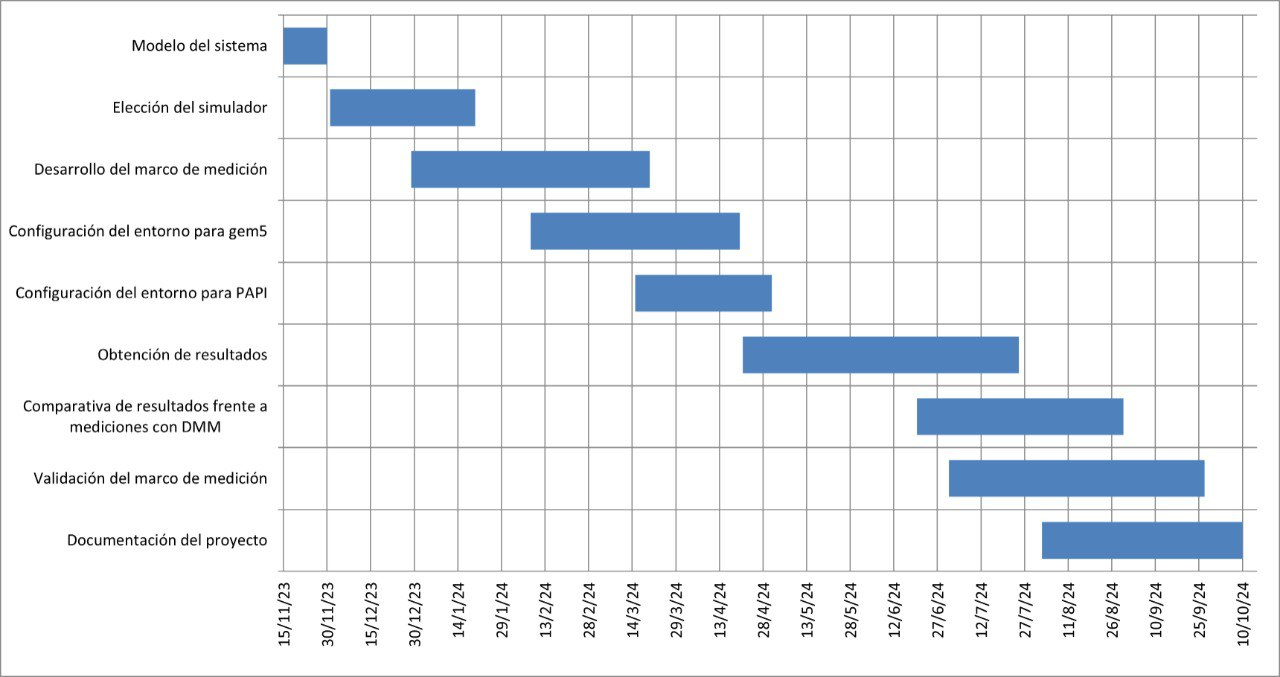
\includegraphics{figs/diagramagantt.png}}
    \caption{Diagrama de Gantt.} 
    \label{fig:diagramaGantt}
\end{figure}


\section{Marco tecnológico}

En esta sección se describirán las herramientas \textit{hardware} y \textit{software} empleadas en el desarrollo de este \ac{TFM}.

\subsection{Herramientas hardware}

\begin{itemize}
    \item \textbf{Ordenador de sobremesa Dell Precision T1700}. Consiste en el equipo utilizado para todas las pruebas realizadas, así como para redactar la documentación de este \ac{TFM}.
    
    \item \textbf{Raspberry Pi 4 (Model B)}. Consiste en la plataforma \textit{hardware} escogida como modelo de pruebas para este trabajo. Sobre este \ac{SBC} se harán las pruebas planteadas. 

    \item \textbf{Cable modificado para realizar mediciones de corriente}. Este cable, diseccionado para poder medir voltaje y corriente, se ha utilizado para medir el consumo de la plataforma de cómputo seleccionada para las pruebas.

    \item \textbf{Multímetro digital (\ac{DMM}) OWON XDM2041}. este multímetro se ha empleado para medir en la realidad la corriente circulante sobre el modelo de pruebas elegido, ante la ejecución de las pruebas planteadas para este trabajo.

    \item \textbf{Multímetro digital (\ac{DMM}) VELLEMAN DVM1200}. este multímetro también se ha empleado las mediciones sobre la plataforma escogida, para reafirmar las mediciones tomadas con el anterior.

\end{itemize}

\subsection{Herramientas software}

\begin{itemize}
    \item \textbf{\href{https://downloads.raspberrypi.org/imager/imager_latest_amd64.deb}{Raspberry Pi Imager}}\footnote{https://downloads.raspberrypi.org/imager/imager\_latest\_amd64.deb}: Se ha utilizado este \textit{software} para obtener la imagen de disco de Raspberry Pi OS que se utilizará dentro de la plataforma Raspberry Pi.
    
    \item \textbf{\href{https://www.python.org/downloads/}{Python}}\footnote{https://www.python.org/downloads/}: Es un conocido lenguaje de programación interpretado, lo que significa que no necesita compilación, permitiendo su funcionamiento en cualquier arquitectura de hardware. En el contexto de este trabajo, se ha utilizado Python 3 en su versión 11.

    \item \textbf{\href{https://code.visualstudio.com/}{Visual Studio Code}}\footnote{https://code.visualstudio.com/}: A lo largo de todo el proyecto, se ha utilizado el ampliamente reconocido \ac{IDE} de Microsoft. Las razones para su elección son numerosas, como la posibilidad de añadir extensiones para el control de versiones con Git, el acceso remoto SSH con visualización de carpetas, un depurador versátil y potente, y una interfaz clara y amigable.
    
    \item \textbf{\href{https://visualstudio.microsoft.com/es/vs/features/cplusplus/}{C}}\footnote{https://visualstudio.microsoft.com/es/vs/features/cplusplus/}: es un famoso lenguaje de programación compilado. Ser compilado significa que requiere de una previa compilación para obtener un archivo binario a ejecutar. C es muy conocido, entre otras cosas, por ser la base del núcleo de Linux. Su éxito se debió en gran parte a su simplicidad y capacidad para realizar operaciones de bajo nivel, manteniendo a la vez un alto grado de abstracción, ideal para el manejo de recursos \textit{hardware}. En este trabajo se ha utilizado para realizar los programas de \textit{benchmark} utilizados para realizar tanto los modelos de consumo en las simulaciones como para la fase de validación.  

    \item \textbf{\href{https://www.gnu.org/software/bash/}{Bash Shell}}\footnote{https://www.gnu.org/software/bash/}: es un popular intérprete de comandos utilizado en sistemas Unix y Linux. Como lenguaje de \textit{scripting}, Bash no requiere de compilación previa, permitiendo la ejecución directa de comandos y \textit{scripts}. Bash es ampliamente conocido por su facilidad para automatizar tareas del sistema, manipular archivos y realizar operaciones repetitivas. En este proyecto, Bash se ha utilizado para filtrado de resultados relacionados con las simulaciones, creación de tablas Excel (ejecutando Python de forma interna) y para la automatización de las pruebas realizadas a lo largo del proyecto.
    
    \item \textbf{\href{https://www.microsoft.com/es-es/microsoft-365/excel}{\ac{MS} Excel}}\footnote{https://www.microsoft.com/es-es/microsoft-365/excel}: Un gestor de hojas de cálculo robusto. En este proyecto, se ha empleado para elaborar tablas con parámetros relevantes relacionados con el consumo de cada componente identificado, así como para realizar cálculos basados en los resultados obtenidos durante las pruebas. También se ha utilizado, en menor medida, la alternativa llamada LibreOffice Calc, de código abierto.

\end{itemize}

\subsection{Herramientas de gestión del proyecto}

\begin{itemize}
    \item \textbf{\href{https://clickup.com/}{ClickUp}}\footnote{https://clickup.com/}: es una herramienta colaborativa de gestión de proyectos en línea, fácil de usar. Permite conocer el estado actual del proyecto, así como planificar con diagramas de Gantt de manera rápida y sencilla, entre otras funciones.
    
    \item \textbf{\href{https://git-scm.com/downloads}{Git}}\footnote{https://git-scm.com/downloads}: es un \textit{Distributed Version Control System} (DVCS, sistema de control de versiones distribuido) que permite mantener un historial del código desarrollado en cada momento, facilitando la recuperación de versiones anteriores si es necesario. En Git, los proyectos se conocen como \emph{repositorios}.
    
    \item \textbf{\href{https://github.com/}{GitHub}}\footnote{https://github.com/}: es una de las diversas plataformas donde los usuarios pueden alojar repositorios Git y registrar los cambios realizados a lo largo del tiempo de manera sencilla. Aunque existen alternativas como BitBucket que son igualmente viables, se ha elegido GitHub debido a la experiencia previa que se tiene con esta plataforma. Para este trabajo, se ha creado un repositorio GitHub, el cual puede accederse desde el siguiente \href{https://github.com/fluctlights/tfm} {enlace}
    
\end{itemize}

\subsection{Herramientas para el desarrollo de la documentación}

\begin{itemize}
    \item \textbf{\href{https://www.latex-project.org/get/}{\LaTeX}}\footnote{https://www.latex-project.org/get/}: es un sistema de procesamiento de documentos basado en TeX que incluye funciones como referencias cruzadas y numeración automática de secciones y ecuaciones, entre otros. Es muy popular en el ámbito académico, principalmente por la alta calidad tipográfica y visual del documento final.
    
    \item \textbf{\href{https://www.overleaf.com/}{Overleaf}}\footnote{https://www.overleaf.com/}: es un editor \textit{online} de \LaTeX, con una interfaz muy intuitiva y unos controles simplificados. Overleaf destaca por su capacidad de colaboración en tiempo real sobre un mismo archivo. Desgraciadamente, es necesaria una cuenta profesional para poder compilar documentos grandes como este TFM, problemática que se ha resuelto creando el documento con este tipo de cuenta y compartiéndolo al resto.
    
    \item \textbf{\href{https://www.tablesgenerator.com/}{Tables Generator}}\footnote{https://www.tablesgenerator.com/}: gracias a esta página se han podido realizar todas las tablas que aparecen en el trabajo, de forma sencilla y muy rápida

    \item \textbf{\href{https://www.drawio.com/}{Drawio}}\footnote{https://www.drawio.com/}: con este editor se han realizado las figuras desarrolladas para este TFM y que  están no integradas directamente en \LaTeX. Permite guardado en la nube o en local, de forma que los archivos estén a salvo, además de utilizar una interfaz sencilla e intuitiva al usuario.
    
    \item \textbf{\href{https://tikzmaker.com/}{TikzMaker}}\footnote{https://tikzmaker.com/}: es un editor de diagramas Tikz que permite realizar esquemas integrados directamente en \LaTeX de forma intuitiva y rápida.

    \item \textbf{\href{http://www.tikzedt.org}{TikzEdt}}\footnote{http://www.tikzedt.org}: es un programa para \ac{MS} Windows que permite la visualización en tiempo real de esquemas Tikz escritos en \LaTeX.
\end{itemize}
